\begin{comment}

	\begin{question}[name=Oppgave, topic=måleusikkerhet]

		\begin{enumerate}[label=\roman*)]

		\end{enumerate}
	\end{question}

	\vspace{0.5cm} % Add space after the solution

	\begin{solution}[name=Løsningsforslag oppgave]

		\begin{figure}[H]
			\centering
			\includegraphics[width=0.7\textwidth]{}
			\caption{}
			\label{fig:}
		\end{figure}
	\end{solution}

	\vspace{0.5cm} % Add space after the solution
\end{comment}



\begin{question}[name=Oppgave, topic=måleusikkerhet]
Lengden på et bord er målt til å være 2 meter. Nøyaktigheten på målinger er $0,2\%$ med en repeterbarhet på $0,05 \%$. Utfør følgende:

	\begin{enumerate}[label=\roman*)]
		\item Beregn total usikkerhet
		\item Beregn absolutt usikkerhet
		\item Beskriv målingen med korrekt usikkerhet
	\end{enumerate}


\end{question}

\vspace{0.5cm} % Add space after the solution

\begin{solution}[name=Løsningsforslag oppgave]
	\begin{enumerate}[label=\roman*)]
	\item Total usikkerhet
\[Total\ usikkerhet = Nøyaktighet + Repeterbarhet = 0,2 \% + 0,05 \% = 0,25 \% \]
	\item Absolutt usikkerhet
\[Absolutt\ usikkerhet = M\text{å}lt verdi \cdot \frac{Total\ usikkerhet}{100}=2 \cdot \frac{0,25}{100}=0,005[m]\]
	\item Beskriv målingen med korrekt usikkerhet
\[(2 \pm 0,005) [m]\]
	\end{enumerate}
\end{solution}

\vspace{0.5cm} % Add space after the solution



\begin{question}[name=Oppgave, topic=måleusikkerhet]
Temperaturen i en ovn måles til $200 [^\circ C]$. Nøyaktigheten i målingen er $0,1 \% $  med en repeterbarhet på $0,002 \%$. Utfør følgende:


	\begin{enumerate}[label=\roman*)]
		\item Total usikkerhet
		\item Absolutt usikkerhet
	\end{enumerate}


\end{question}

\vspace{0.5cm} % Add space after the solution

\begin{solution}[name=Løsningsforslag oppgave]
	\begin{enumerate}[label=\roman*)]
		\item Total usikkerhet
\[Total\ usikkerhet = Nøyaktighet + Repeterbarhet = 0,1 \% + 0,02 \% = 0,12 \% \]
		\item Absolutt usikkerhet
\[Absolutt\ usikkerhet = M\text{å}lt\ verdi \cdot \frac{Usikkerhet}{100}=200 \cdot \frac{0,12}{100}=0,24 [^\circ C]\]
	\end{enumerate}
\end{solution}

\vspace{0.5cm} % Add space after the solution




\begin{question}[name=Oppgave, topic=måleusikkerhet]
For å øke nøyaktigheten på en måling av væskenivå i en tank blir det utført uavhengige målinger etter hverandre. Målingene gir følgende resultater: $49,8[l]$, $50,2[l]$, $50,0[l]$. Nøyaktigheten i målingene er $0,3 \%$ med en repeterbarhet på $0,01 \%$. Utfør følgende:

	\begin{enumerate}[label=\roman*)]
		\item Beregn total usikkerhet
		\item Beregn absolutt usikkerhet
		\item Beskriv målingen med korrekt usikkerhet
	\end{enumerate}


\end{question}

\vspace{0.5cm} % Add space after the solution

\begin{solution}[name=Løsningsforslag oppgave]
	\begin{enumerate}[label=\roman*)]
		\item Finner gjennomsnittsverdien for målingene
\[Gjennomsnitt= \frac{Summen\ av\ alle\ m\text{å}linger}{Antall\ m\text{å}linger}= \frac{49,8+50,2+50,0}{3}=50,0[l]\]

		\item Absolutt usikkerhet

		\item Beskriv målingen med korrekt usikkerhet

	\end{enumerate}
\end{solution}




\begin{question}[name=Oppgave, topic=måleusikkerhet]
En brygger måler volumet av øl ved hjelp av en målesylinder. Målesylinderen har en nøyaktighet på $\pm 0,3 \%$ og en repeterbarhet på $0,01 \%$. Det er utført 10 målinger på en produksjonsenhet med øl, som ga følgende resultat: $50,050[l]$, $49,813[l]$, $50,030[l]$, $50,089[l]$, $49,838[l]$, $50,038[l]$, $49,928[l]$, $50,131[l]$, $50,141[l]$, $49,893[l]$. Utfør følgende:

\begin{enumerate}[label=\roman*)]
	\item Beregn total usikkerhet
	\item Beregn absolutt usikkerhet
	\item Beskriv målingen med korrekt usikkerhet
\end{enumerate}

\end{question}

\vspace{0.5cm} % Add space after the solution

\begin{solution}[name=Løsningsforslag oppgave]
	\begin{enumerate}[label=\roman*)]
	\item Total usikkerhet

		Beregner gjennomsnittet
		\[\mu = 50,050 + 49,813 + 50,030 + 50,089 + 49,838 + 50,038 + 49,928 + 50,131 + 50,141 + 49,893 = 49,995[l]\]

		Total usikkerhet
		\[Total\ usikkerhet = Nøyaktighet + Repeterbarhet = 0,3 + 0,01 = 0,31 \%\]
	\item Absolutt usikkerhet
		\[Absolutt\ usikkerhet = \mu \cdot \frac{Total\ usikkerhet}{100}= 49,995 \cdot \frac{0,31}{100}=0,155 [l]\]

	\item Beskriv målingen med korrekt usikkerhet
		\[(49,995 \pm 0,155) [l]\]

	\end{enumerate}
\end{solution}



\begin{question}[name=Oppgave, topic=måleusikkerhet]
Multimetere vist i Figur \ref{fig:zoyiMul} ble benyttet til å måle en DC-spenning. Instrumentet ga verdien $46,5 [V]$.
	\begin{enumerate}[label=\roman*)]
		\item Med utgangspunkt i data presentert i Figur \ref{fig:zoyiDat} beskriv hvordan det påvirker en måling dersom man bruker et høyere måleområde enn nødvendig
		\item Beregn usikkerhet og vis måleresultatet med usikkerheten, basert på databladet til instrumentet vist i Figur \ref{fig:zoyiDat}.
	\end{enumerate}
Beregn usikkerhet og vis måleresultatet med usikkerheten basert på databladet til instrumentet vist i Figur \ref{fig:zoyiDat}.

	\begin{figure}[H]
		\begin{minipage}[c]{0.45\linewidth}
			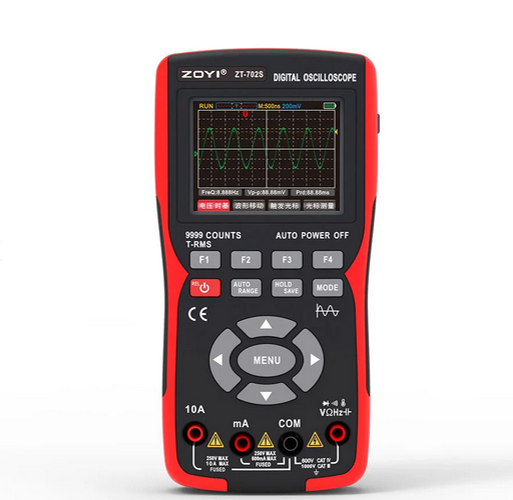
\includegraphics[width=\linewidth]{måleteknikk/figurer/zoyiMultimeter.png}
			\caption{Bilde av måleinstrument}
			\label{fig:zoyiMul}
		\end{minipage}
		\hfill
		\begin{minipage}[c]{0.45\linewidth}
			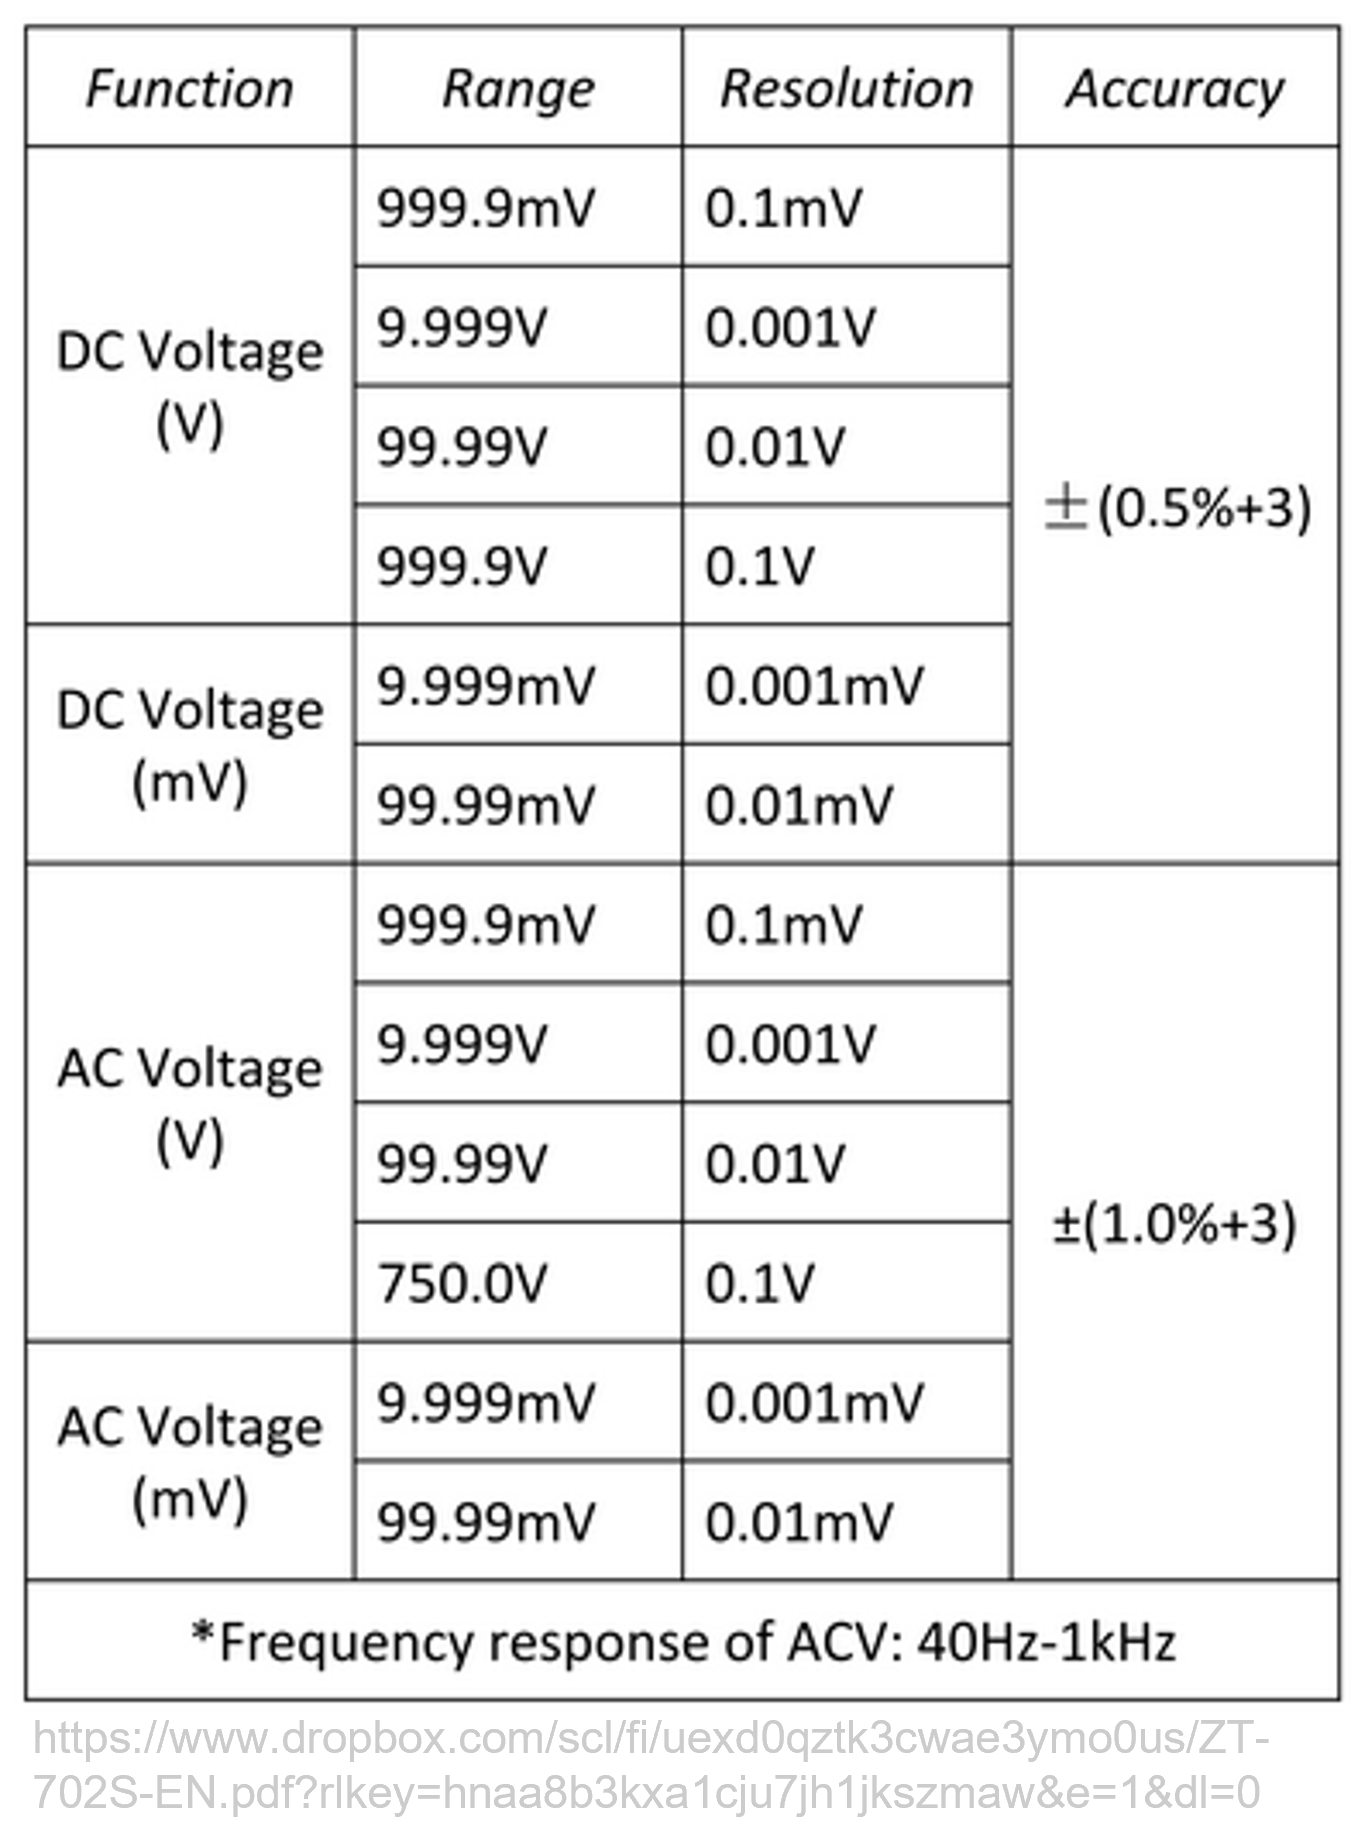
\includegraphics[width=\linewidth]{måleteknikk/figurer/zoyiData.png}
			\caption{Utdrag fra datablad}
			\label{fig:zoyiDat}
		\end{minipage}
	\end{figure}

\end{question}
\vspace{0.5cm} % Add space after the solution

\begin{solution}[name=Løsningsforslag oppgave]
	\begin{enumerate}[label=\roman*)]
	\item Måleinstrumentet vil få en redusert nøyaktighet siden oppløsningen (Resolution) vil reduseres. Dersom man måler $8 [V]$ med måleområde $999,9 [V]$ vil den konstante usikkerheten være på $0,3 [V]$. Hvis man i stede bruker det nærmeste området for målingen som er $9,999 [V]$ vil den konstante usikkerheten være redusert til $0,003 [V]$

	\item Leser av den prosentvise relative usikkerheten fra tabellen til å være $0,5 \%$. Beregner så den absolutte usikkerheten.
	\[Usikkerhet = M\text{å}ling \cdot \frac{Relativ\ usikkerhet}{100}=46,5 \cdot \frac{0,5}{100}=0,235[V]\]

	Leser av den konstante absolutte usikkerheten fra tabellen til å være $3$, og oppløsningen til å være $0,01[V]$.
	\[Usikkerhet_{konst}= Oppløsning \cdot konstant_{usikkerhet} = 3 \cdot 0,01 = 0,03 [V]\]

	Beregner den totale måleusikkerheten
	\[Total\ usikkerhet = Usikkerhet + Usikkerhet_{konst}=0,235+0,03=265 [mV]\]

	Måleresultatet kan beskrive ved:
	\[(46,5 \pm 0,265) [V]\]


\end{enumerate}


\end{solution}